\documentclass[12pt,letterpaper]{article}
\usepackage{fullpage}
\usepackage[top=2cm, bottom=4.5cm, left=2.5cm, right=2.5cm]{geometry}
\usepackage{amsmath,amsthm,amsfonts,amssymb,amscd}
% \usepackage{lastpage}
\usepackage{enumerate}
\usepackage{fancyhdr}
% \usepackage{mathrsfs}
\usepackage{xcolor}
\usepackage{graphicx}
\usepackage{listings}
\usepackage{hyperref}

\usepackage{float}

% define vector
\newcommand{\q}{\underline}
\newcommand{\mt}{\mathrm}

\setlength{\parindent}{0.2in}
\setlength{\parskip}{0.1in}

% Edit these as appropriate
\newcommand\course{Phys 213}
\newcommand\hwnumber{1}                  % <-- homework number
\newcommand\NetIDa{M.-F. Ho}           % <-- NetID of person #1
% \newcommand\NetIDb{netid12038}           % <-- NetID of person #2 (Comment this line out for problem sets)

\pagestyle{fancyplain}
\headheight 35pt
\lhead{\NetIDa}
% \lhead{\NetIDa\\\NetIDb}                 % <-- Comment this line out for problem sets (make sure you are person #1)
\chead{\textbf{\Large Homework 3}}
\rhead{\course \\ \today}
\lfoot{}
\cfoot{}
\rfoot{\small\thepage}
\headsep 1.5em

\newcommand{\Data}{\mathcal{D}}
\newcommand{\xvec}{\boldsymbol{x}}
\newcommand{\Xvec}{\boldsymbol{X}}
\newcommand{\Var}{\textrm{Var}}
\newcommand{\normal}{\textrm{N}}
\newcommand{\xmean}{\langle \xvec \rangle}
\newcommand{\newx}{\tilde{x}}
\newcommand{\integer}{\mathbb{N}}
\newcommand{\thetarv}{\tilde{\theta}}
\newcommand{\phirv}{\tilde{\phi}}

\newcommand{\ml}{m_{\ell}}
\newcommand{\specterms}{^{2S+1}\mathcal{L}^p_\mathcal{J}}

\newcommand{\hi}{\textrm{H\,I}}
\newcommand{\cm}{\textrm{\,cm}}
\newcommand{\cms}{\textrm{\,cm/s}}
\newcommand{\kms}{\textrm{\,km/s}}
\newcommand{\cmcm}{\textrm{\,cm}^{-2}}
\newcommand{\hz}{\textrm{\,s}^{-1}}

\newcommand{\civ}{\textrm{C\,IV}}
\newcommand{\mgii}{\textrm{Mg\,II}}
\newcommand{\caii}{\textrm{Ca\,II}}
\newcommand{\siii}{\textrm{Si\,II}}
\begin{document}

General notations (not always applied):
tildes for variables, no tildes for constants or given values.

\section{radiative transfer}
The differential fom of the equation of radiative transfer is:
\begin{equation}
    \frac{1}{c} \frac{\partial}{\partial t}I_\nu 
    + \hat \Omega \cdot \nabla I_\nu
    + (k_{\nu, s} + k_{\nu, a}) I_\nu 
    = j_\nu + \frac{1}{4\pi} \int_{\Omega} I_{\nu} d\Omega,
\end{equation}
where $j_\nu$ is the emission coefficient, $k_{\nu,s}$  is the scattering opacity, 
$k_{\nu, a}$ is the absorption opacity, and 
$\int_{\Omega} I_{\nu} d\Omega$ is radiation scattered from other direction onto a surface. 

Consider a medium is uniform and isotropic and the radiation is not changing with time:
\begin{equation*}
    \hat \Omega \cdot \nabla I_\nu +   (k_{\nu, s} + k_{\nu, a}) I_\nu 
    = j_\nu + \frac{1}{4\pi} \int_{\Omega} I_{\nu} d\Omega.
\end{equation*} 
By defining source function $S_{\nu} = \frac{j_\nu}{k_{\nu,s} + k_{\nu,a}}$ and ignore the radiation from other places, we have:
\begin{equation*}
    S_\nu 
    = I_\nu + \frac{1}{(k_{\nu, s} + k_{\nu, a})} \hat \Omega \cdot \nabla I_\nu.
\end{equation*} 
If we follow the same procedures as in the textbook:
\begin{equation*}
    d(e^{\tau_\nu} I_{\nu}) = e^{\tau_\nu} S_\nu d\tau_\nu
\end{equation*}
where we set $d\tau_\nu = (k_{\nu, s} + k_{\nu, a}) ds$.
If we do the spherical integration on the LHS, we get $e^{\tau_\nu} \mathbb{E}(I_{\nu}) - I(0)$.
It's no clearly to see the spherical mean of intensity is on LHS, but it is not so clear how to get source function solely on the RHS.
I guess that would require some assumptions that allows the RHS to leave only $S_\nu$.

\section{HI gas and CMB}

\subsection{brightness temperature}
Consider a $\hi$ gas in between CMB radiation and us, the brightness temperature is:
\begin{equation}
    T_B (\tilde \nu=\nu, I_\nu) = \frac{h \nu / k}{\ln{ ( 1 + \frac{2 h \nu^3}{c^2 I_\nu} )  }}.
\end{equation}
Brightness temperature as a function of $\nu$ and $I_\nu$ with the frequency is given:
\begin{equation*}
    \tilde \nu = \nu_{\hi} = \frac{c}{\lambda_{\hi}} = \frac{3 * 10^{10} \cms}{ 21\cm } \simeq 1.5 * 10^{9} \hz.
\end{equation*}

For $\tilde \tau$ is small enough ($\tilde{\tau} = \tau < 0.2$), it is legal to neglect absorption.
We thus have a radiative transfer equation:
\begin{equation}
    I_\nu(\tilde u, \nu_{u\ell}=\nu_{\hi}) = I_\nu(0) +
    \frac{3}{16\pi} A_{u\ell} h \nu_{u\ell} \phi(\tilde u) N(\hi).
    \label{eq:intensity}
\end{equation}
For convenience, we consider line center velocity for the velocity distribution $\phi(\tilde{u} = 0) = \frac{1}{\sqrt{2\pi}}\frac{c}{\nu_{u\ell}}\frac{1}{\sigma_\nu}$.

Some typical values for the 21$\cm$ line are listed in the textbook:
\begin{equation*}
    \begin{split}
        A_{u\ell} &= 2.8843 * 10^{-15} \hz\\
        \nu_{\hi} &= 1420.4 * 10^{6} \hz\\
        \sigma_\nu &\sim \kms\\
        N(\hi) &\simeq 10^{20} \cmcm.
    \end{split}
\end{equation*}

Eq~\ref{eq:intensity} turns out to be:
\begin{equation*}
    I_\nu(\tilde u, \nu_{u\ell}=\nu_{\hi}) = I_\nu(0) +
    \frac{3}{16\pi}
    2.8843 * 10^{-15} \hz
    h 
    1420.4 * 10^{6} \hz
    \frac{1}{\sqrt{2\pi}}\frac{c}{1420.4 * 10^{6}}\frac{1}{\kms}
    10^{20}.    
\end{equation*}

The rest part is to work out the CMB intensity.
Since CMB should be a black body, the LTE condition could be applied here:
\begin{equation}
    I_\nu(0) = B_{CMB}(\tilde \nu = \nu_{CMB}, \tilde{T} = T_{CMB}) = \frac{2h\nu^3}{c^2}\frac{1}{\exp{(h\nu/kT) - 1}},
    \label{eq:intensity_cmb}
\end{equation}
where these values are given:
\begin{equation*}
    \begin{split}
        T_{CMB} &= 2.7255\,K\\
        \nu_{CMB} &= 160.23 * 10^{9} \hz
    \end{split}
\end{equation*}
Combine Eq~\ref{eq:intensity} and Eq~\ref{eq:intensity_cmb}, we arrive:
\begin{equation}
    I_\nu(\tilde{u} = 0) = 3.83 * 10^{-15} + 1.36 * 10^{-17} \simeq 3.84 * 10^{-15},
\end{equation}
with the brightness temperature:
\begin{equation*}
    T_{B} \simeq 6200 \,K.
\end{equation*}
It is much hotter than I believed before.

\subsection{intensity at line center}
From SI unit to Jy is $\times 10^{26}$ and we need to divide $4\pi$ to get solid angle in the nominator of the unit:
\begin{equation*}
    I_\nu = 3 * 10^{7} \textrm{\,Jy\,sr}^{-1}.
\end{equation*}

\section{Doublet metal lines}

\subsection{{\civ} energy levels}
Consider the ground state of electron configuration of {\civ},
\begin{equation*}
    1s^2 2s^1
\end{equation*}
with the spectroscopic term 
\begin{equation*}
    {^2}S_{1/2}.
\end{equation*}

By search the NIST database, we know there are two excited states contribute to {\civ} doublet
\begin{equation*}
    \begin{split}
        {^2P^o_{3/2}}, {{^2}P^o_{1/2}}.
    \end{split}
\end{equation*}
See the diagram below:
\begin{figure}[H]
    \centering
    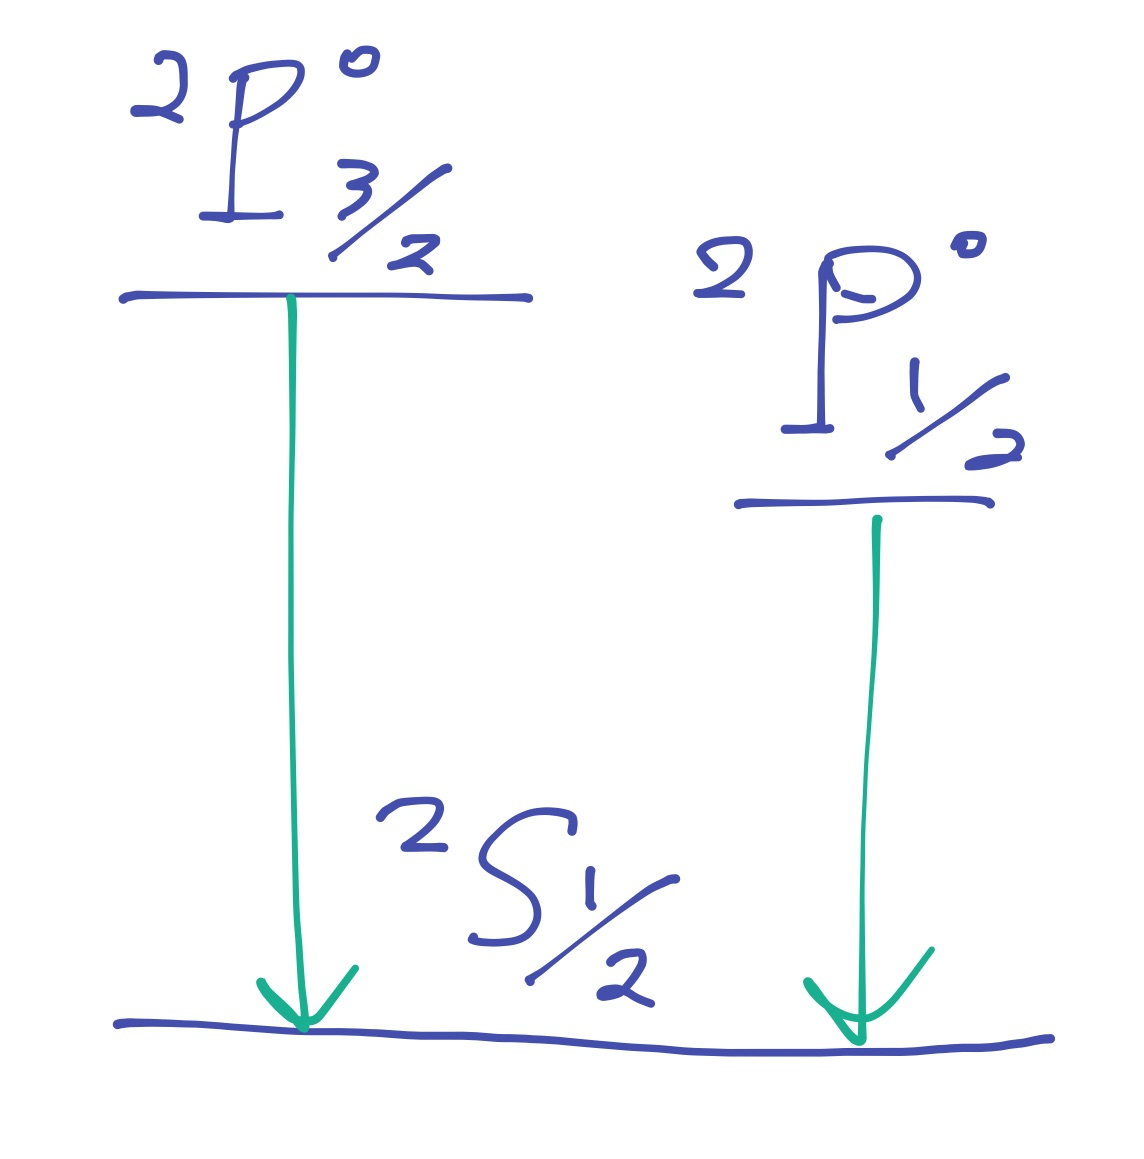
\includegraphics[width=0.5\textwidth]{images/levels.jpg}
\end{figure}


\subsection{optical depth}
The statistical weight is defined as the degeneracy of a given state:
\begin{equation*}
    g = 2 J + 1,
\end{equation*}
so we have $g = 4$ for 1548 {\AA} line and $g = 2$ for 1550 {\AA} line.

According to textbook Eq (9.9), the line-center optical depth is approximated as:
\begin{equation*}
    \tau_0 \propto N_\ell f_{\ell u} \lambda_{\ell u} \frac{1}{b}.
\end{equation*}
The oscillation strength can be written as proportional to the statistical weight, as listed in (6.18) and (6.19):
\begin{equation*}
    f_{\ell u} \propto \frac{g_u}{g_\ell} \frac{1}{\nu_{\ell u}^2} A_{u \ell}.
\end{equation*}
By assuming these two lines have similar Einstein coefficients, here is the final proportionality:
\begin{equation*}
    \tau_0 \propto \frac{g_u}{g_\ell} \lambda_{\ell u}^3
\end{equation*}
which gives:
\begin{equation*}
    \frac{\tau_{1548}}{\tau_{1550}} = 1.99.
\end{equation*}

\subsection{weak lines, EW}
Following the same line of thought, and given that we have (9.28) from the textbook, 
\begin{equation*}
    \frac{W_2}{W_1} =
     \frac{f_{\ell u_2} \lambda_{\ell u_2}}{f_{\ell u_1} \lambda_{\ell u_1}}
\end{equation*}
the ratio of EW should be the same as the ratio of the optical depths
\begin{equation*}
    \frac{W_2}{W_1} = 1.99.
\end{equation*}

\subsection{strong lines, EW}
Following the same line of thought and given that we have (9.29) from the textbook
\begin{equation*}
    \frac{W_2}{W_1} \simeq 
    \left[
        1 + \frac{\ln{(f_{\ell u_2} \lambda_{\ell u_2}/f_{\ell u_1 \lambda_{\ell u_1}})}}{\ln{\tau_{\ell u_1}/\ln{2}}}.
    \right]^{1/2}
\end{equation*}
We already know how to calculate some part of this equation, which gives
\begin{equation*}
    \frac{W_2}{W_1} \simeq 
    \left[
        1 + \frac{\ln{1.99}}{\ln{\tau_{\ell u_1}/\ln{2}}}.
    \right]^{1/2},
\end{equation*}
which is sensitive to what you choose the optical depth for $\tau_{\ell u_1}$. 
For the case $\tau_{\ell u_1} \sim 1.5$, we have $\frac{W_2}{W_1} \simeq 1.5$. 
In a sense we know the ratio is going to be lower.

\subsection{{\mgii} and \caii}
For {\mgii} it has these two energy level transitions which corresponding to 2798 {\AA} and 2803 {\AA}:
\begin{equation*}
    \begin{split}
        {^2}P^o_{3/2} \rightarrow {^2}S_{1/2}\\
        {^2}P^o_{1/2} \rightarrow {^2}S_{1/2};
    \end{split}
\end{equation*}
similarly, for {\caii} we have these two transitions for 3934 {\AA} and 3969 {\AA}:
\begin{equation*}
    \begin{split}
        {^2}P^o_{3/2} \rightarrow {^2}S_{1/2}\\
        {^2}P^o_{1/2} \rightarrow {^2}S_{1/2}.
    \end{split}
\end{equation*}
We clearly notice the changes of the spectroscopic terms from all three ({\civ}, {\mgii}, {\caii}) ions are the same, it just the $n$ for the energy levels are different.
In this case, though we still have $\frac{\lambda_{\ell u_2}^3}{\lambda_{\ell u_1}^3}$ different, but the ratio of statistical weights are the same.
This fact gives that, for weak lines, the ratio of EW are the same $\sim 2$ for all three ions given that the ratio of wavelengths are similar.
While for stronger lines, it depends on the optical depth of one of the lines, but the ratio of EW is not going to be so much different if you look at Fig 9.3, since the term of optical depth is in the log.

\section{composite spectrum}

\begin{figure}[H]
    \centering
    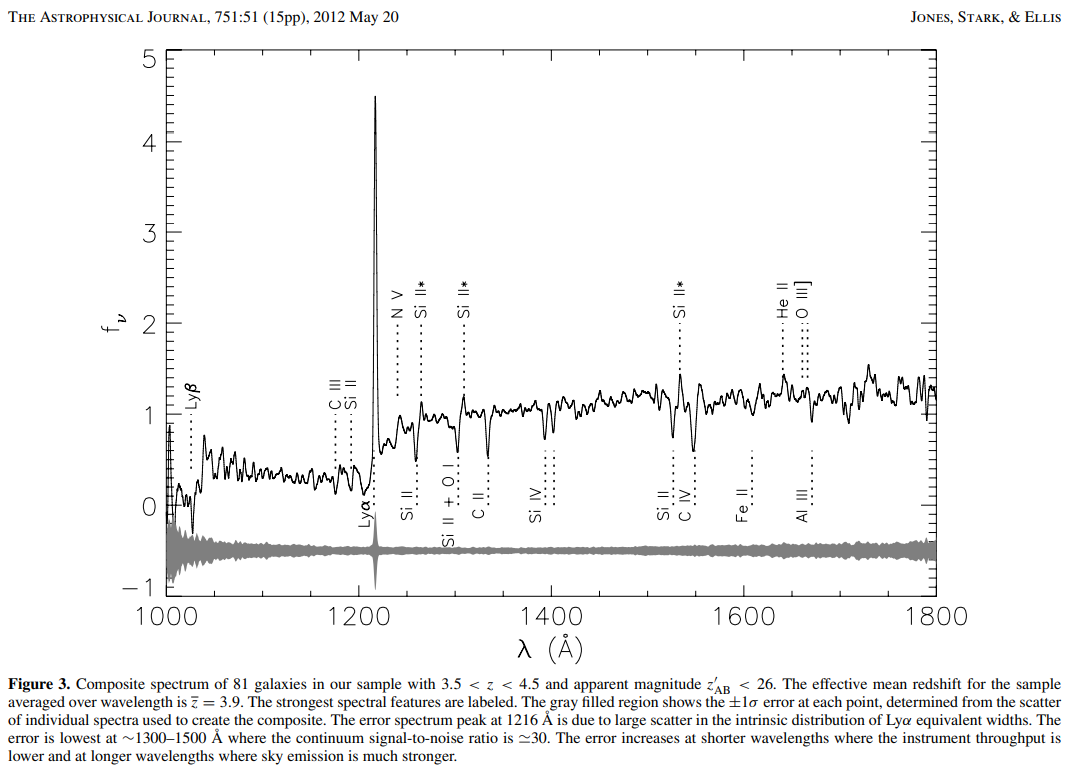
\includegraphics[width=\textwidth]{images/composite_spec.png}
\end{figure}

For {\siii} 1260.4 {\AA},
\begin{equation*}
    \begin{split}
        {^2}D_{3/2} \rightarrow {^2}P^o_{1/2}\\
        A = 2.57 * 10^9 \hz
    \end{split}
\end{equation*}
while for {\siii}* 1264.7 {\AA},
\begin{equation*}
    \begin{split}
        {^2}D_{5/2} \rightarrow {^2}P^o_{1/2}\\
        A = 3.04 * 10^9 \hz.
    \end{split}
\end{equation*}
The apparent difference is the difference in $J$, which means the difference in the degeneracies or the ratio of statistical weights ($g = 2J+1$). 

\subsection{why {\siii}* emission and {\siii} absorption}
The apparent difference between {\siii} and {\siii}* is:
\begin{equation*}
    \begin{split}
        \frac{g_2}{g_1} &= \frac{4}{2}, \textrm{for\,} \siii\\
        \frac{g_2}{g_1} &= \frac{6}{4}, \textrm{for\,} \siii *
    \end{split}
\end{equation*}
This gives no sense at first, but we can think that if the degeneracies is higher than the systems have the tendency to go that direction. 
This sense gives {\siii}* tends to drop to lower level while {\siii} tends to go up to upper level, by comparing these two lines.

But a more reasonable argument is, if we take a look at the transitions of the energy levels:
\begin{equation*}
    \begin{split}
        {\siii}: E_i &= 0.00 \rightarrow E_{f} = 79338.50\\
        {\siii}^*: E_i &= 287.24 \rightarrow E_{f} = 79355.02
    \end{split}
\end{equation*}
Notice it is much easier to go down to ground state for {\siii} than {\siii}*, which makes for sense for {\siii} happens to have more absorptions. 

\end{document}
